%----------------------------------------------------------------------------------------
\chapter{Parallel computing}
%----------------------------------------------------------------------------------------
In this Chapter, a brief overview of the technical aspects of parallel computing is given. Note that this course focuses on the implementation details, like asynchronous programming, see Chapter~\ref{sec:async:coding}; parallel algorithms, see Section~\ref{sec:stl:parallel:algorithms}; and the C++ standard library for parallelism and concurrency (HPX), see Chapter~\ref{sec:hpx}. Note that another option for parallel programming or multi-threaded programming is Open Multi-Processing\link{https://www.openmp.org/} (OpenMP)\index{OpenMP} and some more recent ones Rust\link{https://www.rust-lang.org/}\index{Rust}, Go\link{https://golang.org/}\index{Go}, and Julia language\link{https://julialang.org/}\index{Julia}. However, we provide some details and further references for the technical aspects and hardware details. For a general overview, we refer to~\cite{kumar1994introduction}. Another option are acceleration cards like NVIDIA\textregistered~ or AMD\textregistered~ GPUs.\\

Let us begin with a definition of parallelism: \textit{1)} we need multiple resources which can operate at the same, \textit{2)} we have to have more than one task that can be performed at the same time, \textit{3)} we have to do multiple tasks on multiple resources the same time. First, we have to have multiple resources, \emph{e.g.}\ multiple threads of a computation node at the same time. However, with current hardware architecture this is not an issue. Second, this part is more interesting, since we need some code which is independent of each other and can be executed concurrent. Third, here we want to have overlapping computations and communication on multiple resources. For more details about parallel computing, we refer to~\cite{grama2003introduction,trobec2018introduction}.\\

For the second part of the definition, Amdahl's law\index{Amdahl's law}~\cite{amdahl1967validity} or strong scaling\index{scaling} is important. Amdahl's law is given as
\begin{align}
S = \frac{1}{(1-P) + \frac{P}{N}}
\end{align}
where $S$ is the speed up, $P$ the proportion of parallel code, and $N$ the numbers of threads. Figure~\ref{fig:amdals:law} plots Amdahl's law for different ratios of parallel code. Obviously, for zero percent parallel code, there is no speedup. If the portion to parallel code increases, the speedup increases up to a certain amount of threads. Therefore, the parallel computing with many threads is only beneficial for highly parallelism in our program. For example if our code took 20 hours using a single thread to complete and there in a part of one hour which can not be executed in parallel. Thus, only 19 hours of execution time can be parallized $(p=0.95)$ and independent of the amount of threads we use the theoretical speedup is limited to $S=\sfrac{1}{(1-p)}=20$.\\

\begin{figure}[tb]
\centering
 \begin{tikzpicture}
        \begin{axis}[
            no markers,
            samples=100,
            /pgf/declare function={
            f(\x,\a) = 1. / ((1.-\a)+(\a/x));
       		},
       		grid=both,
       		xlabel=$N$ number of threads,
       		ylabel=$S$ speedup,
       		legend pos=outer north east,
        ]
            % ... and use it here
            \addplot+ [domain=1:2048,azure,thick] {f(x,0)};
            \addlegendentry{$P=0\%$}
            \addplot+ [domain=1:2048,cadetgrey,thick] {f(x,0.5)};
            \addlegendentry{$P=50\%$}
            \addplot+ [domain=1:2048,darkgreen,thick] {f(x,.75)};
            \addlegendentry{$P=75\%$}
            \addplot+ [domain=1:2048,amaranth,thick] {f(x,.90)};
            \addlegendentry{$P=90\%$}
            \addplot+ [domain=1:2048,black,thick] {f(x,.95)};
            \addlegendentry{$P=95\%$}
       \end{axis}
    \end{tikzpicture}
\caption{Plot of Amdahl's law for different parallel portions of the code.}
\label{fig:amdals:law}
\end{figure}

Before we look into different parallelism approaches, we look into the example how to compute the dot product $S = \mathbf{X} \cdot \mathbf{V} = \sum_i^N x_i y_i$ of two vectors $\mathbf{X} = \lbrace x_1,x_2,\ldots,x_n \rbrace$ and $\mathbf{Y} = \lbrace y_1,y_2,\ldots,y_n \rbrace$  in a sequential manner and extend this example to the various parallelism approaches. So we have to compute $S = (x_1y_1) + (x_2y_2) + \ldots + (x_n y_n)$ as shown in the flow chart in Figure~\ref{fig:flow:chart:dot:seq}. In the sequential processing, the first to elements of each vector are multiplied $x_1 \times y_1$ and added to the temporal result. After that the second elements are multiplied and added to the temporal result, and so on. \\

\begin{figure}
\centering
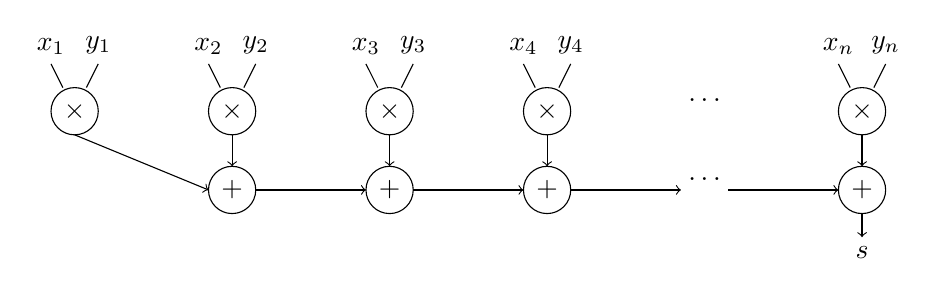
\begin{tikzpicture}
\draw (0,0) circle [radius=0.3] node {$\times$};
\draw (2,0) circle [radius=0.3] node {$\times$};
\draw (4,0) circle [radius=0.3] node {$\times$};
\draw (6,0) circle [radius=0.3] node {$\times$};
\draw (10,0) circle [radius=0.3] node {$\times$};
\node[above] at (8,0) {$\ldots$} ;

\draw (2,-1) circle [radius=0.3] node {$+$};
\draw (4,-1) circle [radius=0.3] node {$+$};
\draw (6,-1) circle [radius=0.3] node {$+$};
\draw (10,-1) circle [radius=0.3] node {$+$};
\node[above] at (8,-1) {$\ldots$} ;

\draw[->](0,-0.3) -- (1.7,-1);
\draw[->](2,-0.3) -- (2,-0.7);
\draw[->](4,-0.3) -- (4,-0.7);
\draw[->](6,-0.3) -- (6,-0.7);
\draw[->](10,-0.3) -- (10,-0.7);

\draw[->](2.3,-1) -- (3.7,-1.);
\draw[->](4.3,-1) -- (5.7,-1.);
\draw[->](6.3,-1) -- (7.7,-1.);
\draw[->](8.3,-1) -- (9.7,-1.);

\draw (-0.15,0.3) -- (-0.3,0.6);
\node[above] at (-0.3,0.6) {$x_1$} ;
\draw (2-0.15,0.3) -- (2-0.3,0.6);
\node[above] at (2-0.3,0.6) {$x_2$} ;
\draw (4-0.15,0.3) -- (4-0.3,0.6);
\node[above] at (4-0.3,0.6) {$x_3$} ;
\draw (6-0.15,0.3) -- (6-0.3,0.6);
\node[above] at (6-0.3,0.6) {$x_4$} ;
\draw (10-0.15,0.3) -- (10-0.3,0.6);
\node[above] at (10-0.3,0.6) {$x_n$} ;

\draw (0.15,0.3) -- (0.3,0.6);
\node[above] at (0.3,0.6) {$y_1$} ;
\draw (2+0.15,0.3) -- (2+0.3,0.6);
\node[above] at (2+0.3,0.6) {$y_2$} ;
\draw (4+0.15,0.3) -- (4+0.3,0.6);
\node[above] at (4+0.3,0.6) {$y_3$} ;
\draw (6+0.15,0.3) -- (6+0.3,0.6);
\node[above] at (6+0.3,0.6) {$y_4$} ;
\draw (10+0.15,0.3) -- (10+0.3,0.6);
\node[above] at (10+0.3,0.6) {$y_n$} ;

\draw[->](10,-1.3) -- (10,-1.6);
\node[below] at (10,-1.6) {$s$} ;
\end{tikzpicture}
\caption{Flow chart of the sequential evaluation of the dot product of two vectors. }
\label{fig:flow:chart:dot:seq}
\end{figure}

The first parallelism approach is the pipeline parallelism\index{pipeline parallelism}~\cite{ramamoorthy1977pipeline}. The pipeline parallelism is used in vector processors and in execution pipelines in all general microprocessors. Let us look into some example of from the automotive industry. First, the body of the car is assembled. Second, workers assemble the chassis. Third, workers add the engine into the chassis. Next, the steering wheel is added and many more steps until the car is finally assembled. TO make this process efficient, the workers assembling the chassis do not wait until the last step is finalized before they start working on the next chassis. Side note this is similar to the assembly line introduced bu Henry Ford to enable mass production of cars~\cite{watts2009people}.\\

Figure~\ref{fig:dataflow:pipeline} shows the data flow chart for the pipeline parallelism. In the first step, the values $x_1$ and $y_1$ are read from memory. In the second step the values are multiplied. In the last step the result of the multiplication is added to the variable $S$. However, the other threads do not idle until the result is computed and do a previous step if possible. Meaning if the multiplication at stage two is happening, another thread starts to get the next values. For more details, we refer to~\cite{quinn2003parallel}. \\


\begin{figure}[tb]
\centering
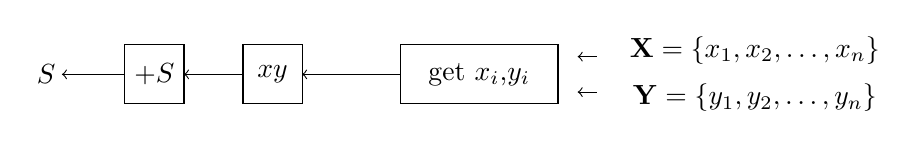
\begin{tikzpicture}
\draw (0,0) rectangle ++(0.75,0.75) node[pos=.5] {$+S$};
\draw (1.5,0) rectangle ++(0.75,0.75) node[pos=.5] {$xy$}; 
\draw (3.5,0) rectangle ++(2,0.75) node[pos=.5] {\text{get} $x_i$,$y_i$};

\node[above] at (8,0.5*0.75) {$\mathbf{X} = \lbrace x_1,x_2,\ldots,x_n \rbrace$} ;
\node[below] at (8,0.5*0.75) {$\mathbf{Y} = \lbrace y_1,y_2,\ldots,y_n \rbrace$} ;
\node at (-1,0.5*0.75) {$S$} ;

\draw[<-](-0.8,0.5*0.75) -- (0,0.5*0.75) ;
\draw[<-](0.75,0.5*0.75) -- (1.5,0.5*0.75) ;
\draw[<-](2.25,0.5*0.75) -- (3.5,0.5*0.75) ;
\draw[<-](5.75,0.8*0.75) -- (6,0.8*0.75) ;
\draw[<-](5.75,0.2*0.75) -- (6,0.2*0.75) ;
\end{tikzpicture}
\caption{Flow chart for the pipeline processing for the dot product.}
\label{fig:dataflow:pipeline}
\end{figure}

The second parallelism approach is the Single instructions and multiple data (SIMD)\index{SIMD}\index{single instructions and multiple data}. SIMD is part of Flynn's taxonomy, a classification of computer architectures, proposed by Michael J. Flynn in 1966~\cite{flynn1972some,duncan1990survey}. Following aspects are relevant 
\begin{itemize}
\item All perform same operation at the same time
\item But may perform different operations at different times
\item Each operates on separate data
\item Used in accelerators on microprocessors
\item Scales as long as data scales.
\end{itemize}
\vspace{0.25cm}
Figure~\ref{fig:reduction:tree:simd} shows the reduction tree for the dot product computation. For this parallelism approach all threads perform the same operation at the same time. In our case all available threads multiply two values at the first level. Second one of these threads add the partial results. Until not all elements are read from the vector these steps are repeated. The last step is to accumulate all partial results and the final result is available. For example previous CUDA architectures were designed this way and introducing branching had some effect on the performance. Newer CUDA architectures perform better here and these things are explained in following talk\link{https://youtu.be/5vr7ItjyIH8}.

\begin{figure}[tb]
\centering
  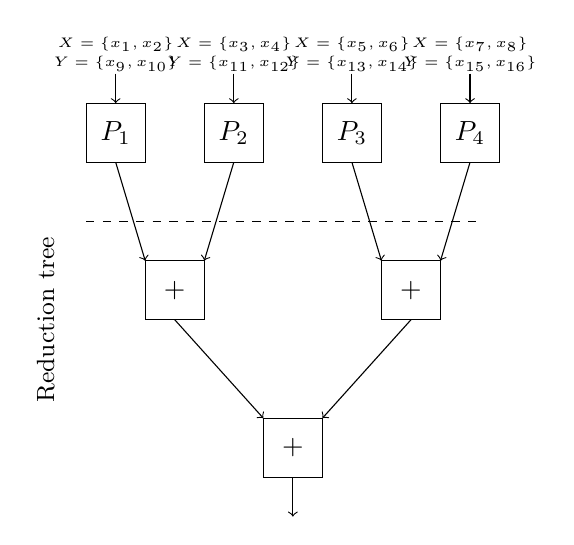
\begin{tikzpicture}
   \draw (0,0) rectangle ++(0.75,0.75) node[pos=.5] {$P_1$}; 
   \draw (1.5,0) rectangle ++(0.75,0.75) node[pos=.5] {$P_2$}; 
   \draw (3,0) rectangle ++(0.75,0.75) node[pos=.5] {$P_3$}; 
   \draw (4.5,0) rectangle ++(0.75,0.75) node[pos=.5] {$P_4$}; 
   
   \draw (0.75,-2) rectangle ++(0.75,0.75) node[pos=.5] {$+$}; 
   \draw (3.75,-2) rectangle ++(0.75,0.75) node[pos=.5] {$+$}; 
   
   \draw (2.25,-4) rectangle ++(0.75,0.75) node[pos=.5] {$+$}; 
   
   \draw[->] (0.75+0.5*0.75,-2) -- (2.25,-4+0.75) ;
   \draw[->] (3.75+0.5*0.75,-2) -- (3,-4+0.75) ;
   
   \draw[->] (1.5+0.5*0.75,0) -- (1.5,-2+0.75) ;
   \draw[->] (0.5*0.75,0) -- (0.75,-2+0.75) ; 
   
   \draw[->] (3+0.5*0.75,0) -- (3.75,-2+0.75) ;
   \draw[->] (4.5+0.5*0.75,0) -- (4.5,-2+0.75) ; 
   
   \draw[->] (2.25+0.5*0.75,-4) -- (2.25+0.5*0.75,-4.5) ; 
   
   \draw[dashed] (0,-0.75) -- (5,-0.75) ;
   \node[below,rotate=90] at (-.75,-2) {\small Reduction tree}; 
   
   \node at (0.5*0.75,1.5) {\tiny $X=\lbrace x_1,x_2 \rbrace$};
   \node at (0.5*0.75,1.25) {\tiny $Y=\lbrace x_9,x_{10} \rbrace$};
   \node at (1.5+0.5*0.75,1.5) {\tiny $X=\lbrace x_3,x_4 \rbrace$};
   \node at (1.5+0.5*0.75,1.25) {\tiny $Y=\lbrace x_{11},x_{12} \rbrace$};
   \node at (3.+0.5*0.75,1.5) {\tiny $X=\lbrace x_5,x_6 \rbrace$};
   \node at (3.+0.5*0.75,1.25) {\tiny $Y=\lbrace x_{13},x_{14} \rbrace$}; 
   \node at (4.5+0.5*0.75,1.5) {\tiny $X=\lbrace x_7,x_8 \rbrace$};
   \node at (4.5+0.5*0.75,1.25) {\tiny $Y=\lbrace x_{15},x_{16} \rbrace$};
   
   \draw[->] (0.5*0.75,1.125) -- (0.5*0.75,0.75) ;
   \draw[->] (1.5+0.5*0.75,1.125) -- (1.5+0.5*0.75,0.75) ;
   \draw[->] (3.+0.5*0.75,1.125) -- (3.+0.5*0.75,0.75) ;
   \draw[->] (4.5+0.5*0.75,1.125) -- (4.5+0.5*0.75,0.75) ;
   \end{tikzpicture}
   \caption{Reduction tree for the dot product using single instructions and multiple data.}
   \label{fig:reduction:tree:simd}
\end{figure}

%----------------------------------------------------------------------------------------
\subsection*{Memory access}
\index{memory access}
%----------------------------------------------------------------------------------------
For parallel computing, the memory access scheme is important to understand performance behavior. If we initialize for example the two vectors in the dot product example, some space in the memory is reserved and filled with the values. For the computation of the dot product these elements have to be read from memory and the CPU is doing the computation. In a layman's view the CPU is connected to the memory via a so-called bus. Depending on the bus's architecture the access time differs and may have effects on the performance if there is a switch from one CPU to the second CPU.\\

The first memory access scheme is uniform memory access (UMA), see Figure~ref{fig:memory:uma},  where all memory is attached to one bus and all CPU are attached to the same bus. Therefore, the memory access times are the same for all CPU. So we do not see any effect if we switch from one two two CPU. The second memory access scheme is non-uniform memory access (NUMA), see Figure~\ref{fig:memory:numa}. Here, the access time to the memory depends on the memory location relative to the CPU. Thus, local memory access is fast and non-local memory access has some overhead. For more details about memory access, we refer to~\cite{el2005advanced,hager2010introduction}.

\begin{figure}
\centering
\begin{minipage}[c]{0.45\textwidth}
\centering
   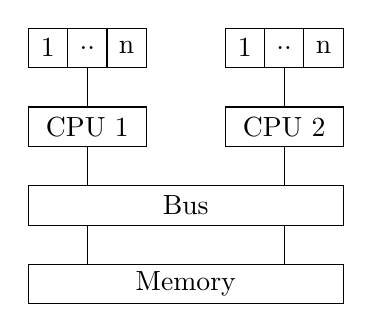
\begin{tikzpicture}
%Threads
\draw (0,3) rectangle (.5,3.5) node[pos=.5] {1};
\draw (0.5,3) rectangle (1.0,3.5) node[pos=.5] {..};
\draw (1.,3) rectangle (1.5,3.5) node[pos=.5] {n};

\draw (2.5,3) rectangle (3.,3.5) node[pos=.5] {1};
\draw (3.,3) rectangle (3.5,3.5) node[pos=.5] {..};
\draw (3.5,3) rectangle (4,3.5) node[pos=.5] {n};

\draw (0.75,2.5) -- (0.75,3.);
\draw (3.25,2.5) -- (3.25,3.);

%BUS
\draw (0,1) rectangle (4,1.5) node[pos=.5] {Bus};


%CPU
\draw (0,2) rectangle (1.5,2.5) node[pos=.5] {CPU 1};
\draw (2.5,2) rectangle (4,2.5) node[pos=.5] {CPU 2};
\draw (0.75,2) -- (0.75,1.5);
\draw (3.25,2) -- (3.25,1.5);

%Memory
\draw (0,0) rectangle (4,0.5) node[pos=.5] {Memory};
\draw (0.75,.5) -- (0.75,1.);
\draw (3.25,.5) -- (3.25,1.);
\end{tikzpicture}
    \caption{Uniform memory access (UMA)\index{uniform memory access}\index{UMA}}
    \label{fig:memory:uma}
\end{minipage}
\hfill
\begin{minipage}[c]{0.45\textwidth}
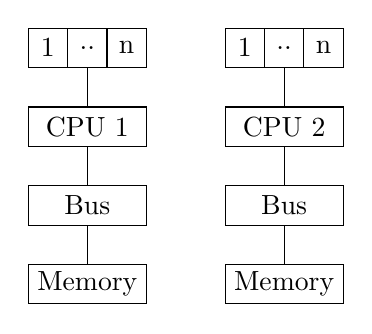
\begin{tikzpicture}
%Threads
\draw (0,3) rectangle (.5,3.5) node[pos=.5] {1};
\draw (0.5,3) rectangle (1.0,3.5) node[pos=.5] {..};
\draw (1.,3) rectangle (1.5,3.5) node[pos=.5] {n};

\draw (2.5,3) rectangle (3.,3.5) node[pos=.5] {1};
\draw (3.,3) rectangle (3.5,3.5) node[pos=.5] {..};
\draw (3.5,3) rectangle (4,3.5) node[pos=.5] {n};

\draw (0.75,2.5) -- (0.75,3.);
\draw (3.25,2.5) -- (3.25,3.);

%BUS
\draw (0,1) rectangle (1.5,1.5) node[pos=.5] {Bus};
\draw (2.5,1) rectangle (4,1.5) node[pos=.5] {Bus};

%CPU
\draw (0,2) rectangle (1.5,2.5) node[pos=.5] {CPU 1};
\draw (2.5,2) rectangle (4,2.5) node[pos=.5] {CPU 2};
\draw (0.75,2) -- (0.75,1.5);
\draw (3.25,2) -- (3.25,1.5);

%Memory
\draw (0,0) rectangle (1.5,0.5) node[pos=.5] {Memory};
\draw (2.5,0) rectangle (4,0.5) node[pos=.5] {Memory};
\draw (0.75,.5) -- (0.75,1.);
\draw (3.25,.5) -- (3.25,1.);
\end{tikzpicture}
    \caption{Non-uniform memory access (NUMA)\index{non-uniform memory access}\index{NUMA}}
    \label{fig:memory:numa}
\end{minipage}

\end{figure}



%----------------------------------------------------------------------------------------
\section{Caution: Data races and dead locks}
\label{sec:deadlocks}
%----------------------------------------------------------------------------------------
Remember with great power comes great responsibility! Meaning with shared memory parallelism you add an additional source of error to your code. When using parallel execution policy, it is the programmer's responsibility to avoid
\begin{itemize}
\item data races
\item race conditions
\item deadlocks.
\end{itemize} 
Let us look into some code examples for these kind of errors. A data race\index{data race} exists when multi-threaded (or otherwise parallel) code that would access a shared resource could do so in such a way as to cause unexpected results. Listing~\ref{code:data:race} shows an example for a data race for the variable \cpp{sum}. Since the parallel execution policy is used, multiple threads can access the variable \cpp{sum} at the same time which means that not all threads can write to the variable. Thus, the result is might not correct. There are two solutions to avoid the data race. First, the atomic library\link{https://en.cppreference.com/w/cpp/atomic/atomic}. The atomic library\footnote{\tiny\url{https://en.cppreference.com/w/cpp/atomic}} provides components for fine-grained atomic operations allowing for lockless concurrent programming. Each atomic operation is indivisible with regards to any other atomic operation that involves the same object. Atomic objects are free of data races. Listing~\ref{code:datarace:atomic} shows the solution using \cpp{std::atomic:<int>}\link{https://en.cppreference.com/w/cpp/atomic/atomic}. The second solution is shown in Listing~\ref{code:datarace:mutex}. Here, the \cpp{std::mutex} class is used to avoid the data race. The mutex class\link{https://en.cppreference.com/w/cpp/thread/mutex} is a synchronization primitive that can be used to protect shared data from being simultaneously accessed by multiple threads. In Line~4 a \cpp{std::mutex m;} is generated. In Line~8 the lock of the code is started by using \cpp{m.lock();} and in Line~10 the lock is released by using \cpp{m.unlock();}.

\begin{exercise}
Give a definition for \cpp{std::atomic} and \cpp{std::mutex} in your own words. 
\end{exercise}

Another source of error is the race condition\index{race condition} where a check of a shared variable within a parallel execution and another thread could change this variable before it is used. Listing~\ref{code:racecondition} shows the solution to avoid the race condition.  Imagine the code without the \cpp{std::mutex} and the implication to get a wrong result. In the code there is a check if \cpp{x} is equal to 5 and a special treatment of the computation in this case. Now in Line~4 it was true that \cpp{x} was equal to five and the thread enters the \cpp{if} branch. However, in between another thread could change the value of \cpp{x} and not \cpp{y = 5 *2} is computed. By using the mutex this situation is avoided.

\begin{exercise}
Explain a data race in your own words and explain why a \cpp{std::mutex} avoids the data race.
\end{exercise}

\begin{lstlisting}[language=c++,caption={Example code and Solution for a data race.\label{code:data:race}},float,floatplacement=tb]
//Compute the sum of the array a in parallel
int a[] = {0,1,2,3,4};
int sum = 0;
std::for_each(std::execution::par, 
              std::begin(a), 
              std::end(a), [&](int i) {
  sum += a[i]; // Error: Data race
});
\end{lstlisting}


\begin{lstlisting}[language=c++,caption={Solution to avoid the data race using \cpp{std::atomic}.\label{code:datarace:atomic}},float,floatplacement=tb]
//Compute the sum of the array a in parallel
int a[] = {0,1};
std::atomic<int> sum{0};
std::for_each(std::execution::par, 
              std::begin(a), 
              std::end(a), [&](int i) {
  sum += a[i]; 
});
\end{lstlisting}

\begin{lstlisting}[language=c++,caption={Solution to avoid the data race using \cpp{std::mutex}.\label{code:datarace:mutex}},float,floatplacement=tb]
//Compute the sum of the array a in parallel
int a[] = {0,1};
int sum = 0;
std::mutex m;
std::for_each(std::execution::par, 
              std::begin(a), 
              std::end(a), [&](int i) {
  m.lock();
  sum += a[i];
  m.unlock(); 
});
\end{lstlisting}


\begin{lstlisting}[language=c++,caption={Example for the race condition.\label{code:racecondition}},float,floatplacement=tb]
std::mutex m;

m.lock();
if (x == 5)  // Checking x
{
   // Different thread could change x 
      
   y = x * 2; // Using x
}
m.unlock();
// Now it is sure that y will be 10
\end{lstlisting}


A deadlock\index{deadlock} describes a situation where two or more threads are blocked forever and waiting for each others. Following example taken from\link{https://docs.oracle.com/javase/tutorial/essential/concurrency/deadlock.html} explains a deadlock nicely. \\

\textit{Alphonse and Gaston are friends, and great believers in courtesy. A strict rule of courtesy is that when you bow to a friend, you must remain bowed until your friend has a chance to return the bow. Unfortunately, this rule does not account for the possibility that two friends might bow to each other at the same time.}

\begin{exercise}
The implementation of this examples is available on GitHub\link{https://github.com/diehlpkteaching/ParallelComputationMathExamples/blob/master/chapter10/lecture6-deadlock.cpp.ipynb}. Play around with the example and try to understand why the code results in a deadlock. 
\end{exercise}

%----------------------------------------------------------------------------------------
\chapter{Asynchronous programming}
\label{sec:async:coding}
\index{future}
\index{async}
\index{C++!asynchronous programming}
%----------------------------------------------------------------------------------------
A different concept for shared memory parallelism is asynchronous programming~\cite{williams2012c++}. Before we look into asynchronous programming, we look again into the concept of serial programming. Figure~\ref{fig:async:dependencygraph} shows the dependency graph for one computation and one can see that we can compute $P$ and $X$ independent and only $H$ depends on both of them. Listing~\ref{code:serial:dependency} shows the serial computation of the dependency graph. Each line of code is executed line by line Each time a function is called the code waits until the function finishes. Thus, we can not compute $P$ and $X$ independently, even if the data is independent. 

\vspace{0.25cm}
\begin{minipage}{\linewidth}
\begin{minipage}{0.45\linewidth}
\centering
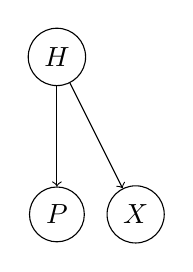
\begin{tikzpicture}
\node (a) [draw,circle] at (0,2) {$H$};
\node (b) [draw,circle] at (0,0) {$P$};
\node (c) [draw,circle] at (1,0) {$X$};
\draw [->] (a) -- (b);
\draw [->] (a) -- (c);
\end{tikzpicture}
\captionof{figure}{Example dependency graph}
\label{fig:async:dependencygraph}
\end{minipage}
\hfill
\begin{minipage}{0.5\linewidth}
\begin{lstlisting}[language=c++,caption={Synchronous execution of the dependency graph.\label{code:serial:dependency}}]
auto P = compute();
auto X = compute();
auto H = compute(P,X);
\end{lstlisting}
\end{minipage}
\end{minipage}
\vspace{0.25cm}

To executed lines asynchronously the C++ language provides the \cpp{std::async}\link{https://en.cppreference.com/w/cpp/thread/async}\index{async}\index{C++!async} expression provided by the \cpp{#include <future>}. Listing~\ref{code:async:dependency} shows the asynchronous implementation of the dependency graph in Figure~\ref{fig:async:dependencygraph}. Line~2 shows the usage of \cpp{std::async} for the function \cpp{compute}. The first argument is the name of the function or a lambda expression, see Section~\ref{sec:lambda:function}. Because we used \cpp{std::async} this line of code is executed in the background on a different thread and the next line of code is executed, even if the result of the computation is not ready yet. Therefore, \cpp{std::async} return a \cpp{std::future<int>}\link{https://en.cppreference.com/w/cpp/thread/future}\index{future}\index{C++!future} object provided by the \cpp{#include <future>} header which is a template and contains the return type of the function which is in this example the \cpp{int} data type. In Line~4, the computation of $X$ is started on another thread. Such that both computations happens at the same time. In Line~7--9 the results of the asynchronous function call are gathered, since these are needed to compute $H$. With the \cpp{.get()} function a barrier is introduced and the line of codes waits until the computation is ready. In our case, we can wait since we need the two results to compute the last one. Meaning that Line~8 is only executed if the computation in Line~2 has finished. Following synchronization features are available:
\begin{itemize}
\item \lstinline|.get()| returns the result of the functions and wait until the computation finished
\item \lstinline|.wait()|\link{https://en.cppreference.com/w/cpp/thread/future/wait} waits until the computation finished
\item \lstinline|.wait_for(std::chrono::seconds(1))|\link{https://en.cppreference.com/w/cpp/thread/future/wait_for} returns if it is not available for the specified timeout duration 
\item \lstinline|.wait_until(std::chrono::seconds(1))|\link{https://en.cppreference.com/w/cpp/thread/future/wait_until} waits for a result to become available. It blocks until specified timeout time has been reached or the result becomes available, whichever comes first. 
\end{itemize}

\begin{lstlisting}[language=c++,caption={Asynchronous execution of the dependency graph.\label{code:async:dependency}},float,floatplacement=tb]
// Compute P
std::future<int> f1 = std::async(compute);
// Compute X
auto f2 = std::async(compute);

// Gather the results
int P = f1.get();
int X = f2.get();

// Compute the dependent result H
std::cout << compute(P,X) << std::endl;
\end{lstlisting}

\section*{Example}
Let us look into one example to show the parallelism using asynchronous programming for the Taylor series. The approximation of the $\sin$ function is given as
\begin{align}
\sin(x) = \sum\limits_{n=0}^N (-1)^{n-1} \frac{x^{2n}}{(2n)!} 
\label{eq:sin:taylor}
\end{align}
One approach to parallize the above function using two threads is:
\begin{enumerate}
\item Split $n$ into slices, e.g. 2 times $\sfrac{n}{2}$ for two threads
\item Start two times \lstinline|std::async| where each thread computes $\sfrac{n}{2}$
\item Use the two futures to synchronize the results
\item Combine the two futures to obtain the result.
\end{enumerate}
To distribute $n$ into slices, we need to write the sum in Equation~\eqref{eq:sin:taylor} as
\begin{align}
\sum\limits_{n=begin}^{end} (-1)^{n-1} \frac{x^{2n}}{(2n)!} \text{.}
\end{align}
Listing~\ref{code:async:taylor} shows how to implement the function to splice the computation of the Taylor series, see Line~5--14. In Line~18--19 the two splices $\sfrac{n}{2}$ are launched from $0$ up to $49$ on the first thread and from $50$ up to $99$ on the second thread. In Line~22 the result is gathered and finally the accumulated result is evaluated. For more details, we refer to following talk\link{https://www.youtube.com/watch?v=js-e8xAMd1s}.

To compile the code using asynchronous programming, we need to add \lstinline|-pthread| to our compiler to use the POSIX threads to launch the functions asynchronous (\lstinline|std::async|). More details about POSIX\index{POSIX} threads~\cite{butenhof1997programming,kleiman1996programming}.




\begin{lstlisting}[language=c++,caption={Asynchronous computation of the $\sin$ function using a Taylor series.\label{code:async:taylor}},float,floatplacement=tb]
#include <future>
#include <iostream>

// Function to compute portion of the Taylor series
double taylor(size_t begin, size_t end, 
double x,size_t n){
double res = 0;

	for( size_t i = begin ; i < end ; i++)
	{
	  res += pow(-1,i-1) * pow(x,2*n) / factorial(2*n);
	} 
return res;
}

int main(){
	// Asynchronous computation using two slices
	auto f1 = std::async(taylor,0,49,2,100); 
	auto f2 = std::async(taylor,50,99,2,100); 
	
	// Gather the result
	double result = f1.get() + f2.get();

	// Print the result
	std::cout << "sin(2)= " res << std::endl;

	return 0;
}
\end{lstlisting}


%----------------------------------------------------------------------------------------
\chapter{Distributed Programming}
\label{sec:distributed:programming}
%----------------------------------------------------------------------------------------
\begin{figure}[tb]
\centering
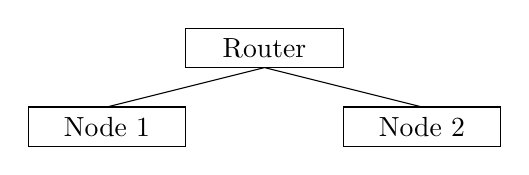
\begin{tikzpicture}
\draw (0,3) rectangle (2,3.5) node[pos=.5] {Node 1};
\draw (4,3) rectangle (6,3.5) node[pos=.5] {Node 2};

\draw (2,4) rectangle (4,4.5) node[pos=.5] {Router};
\draw (1,3.5) -- (3,4) ;
\draw (5,3.5) -- (3,4) ;
\end{tikzpicture}
\caption{Sketch of the components of a distributed system. We have multiple computational nodes which are connected to a router or switch and they send messages to each other over the network. In that specific example, we have two nodes connected to one router. For the network connection Ethernet or more efficient Mellanox\textregistered~InfiBand\texttrademark~ is used. A common standard to send and receive messages is the Message Passing Interface (MPI) standard.}
\label{fig:distributed:nodes}
\end{figure}
Previously, we considered shared memory parallelism which means we only considered one physical computational node. Now, we will look into distributed programming because the memory or the computational resources of one physical computational node are not sufficient. A good definition for distributed computing is given in~\cite{van2002distributed}: ``A distributed system is a system whose components are located on different networked computers, which communicate and coordinate their actions by passing messages to one another from any system''. Fore more details about distributed systems, we refer to~\cite{van2002distributed}. Figure~\ref{fig:distributed:nodes} sketches the components of a distributed system. We have multiple computational nodes which are connected to a router or switch and they send messages to each other over the network. In that specific example, we have two nodes connected to one router. For the network connection Ethernet or more efficient Mellanox\textregistered~InfiBand\texttrademark~ is used. A common standard to send and receive messages is the Message Passing Interface\index{Message Passing Interface} (MPI)\index{MPI} standard. Here, we have the similar definition that the MPI standard specifies the API and several implementations, \emph{e.g.}\ OpenMPI\link{https://www.open-mpi.org/} or mpich2\link{https://www.mpich.org/}, are available. Next to these open source implementations there are commercial implementations, \emph{e.g.}\ IntelMPI and IBM Spectrum-MPI available. For more details about MPI programming, we refer to~\cite{gropp1999using}. Listing~\ref{code:mpi:example} shows some small example for sending messages and receiving messages. In Line~\ref{code:mpi:example:init} the MPI environment is initialized. In Line~\ref{code:mpi:example:rank} the rank or if of the node where the code is executed is determined. Some common convention is that node with rank zero is the head node and does the synchronization. In Line~\ref{code:mpi:example:receive} the head node waits for receiving some message and in Line~\ref{code:mpi:example:send} the other node is sending some message to the head node. Note that the MPI library has only a C interface and not C++ interface is available yet. The intention of this example was to show you how to use the low-level API of the MPI library and later we will see in Section~\ref{sec:hpx::distributed} that HPX provides some abstraction layer to send and receive messages. One common term in high performance computing is \texttt{MPI+X}\index{MPI+X} which means that the MPI is used to send and receive messages over the network and \texttt{X} is used for the parallelism on each of the computational nodes. For example OpenMP is used for shared memory parallelism for CPUs and CUDA\texttrademark~\index{CUDA} or HIP\texttrademark\link{https://rocmdocs.amd.com/en/latest/ROCm_Compiler_SDK/ROCm-Compiler-SDK.html}~\index{HIP} are used for NVIDIA\texttrademark~ or AMD\texttrademark~ acceleration cards, respectively. Fore more details about CUDA\texttrademark\link{https://docs.nvidia.com/cuda/cuda-c-programming-guide/index.html}~ programming, we refer to~\cite{sanders2010cuda}. However, for the \texttt{MPI+X} approach the programmer has to deal with different API for the distributed and shared memory approach. Furthermore, for heterogeneous systems the programmer has to deal with a third API for the acceleration cards. Sometimes the different APIs result in duplicated code since one would need to implement the same piece of code using OpenMP and CUDA for example. Fore more details on how to overcome these issue, we refer to~\cite{7543422}. One attempt to provide a unified API for various shared parallelism options is kokkos~\cite{10.1016/j.jpdc.2014.07.003}\index{kokkos}. Some alternative framework is libfabric~\cite{7312664} which was integrated within HPX. We could show that using synchronous communication suing MPI was up to a factor of three slower than asynchronous communication using libfabric~\cite{daiss2019piz}.


\begin{lstlisting}[language=c++,caption={Small Message Passing Interface example to send and receive messages.\label{code:mpi:example}},float,floatplacement=tb,escapechar=|]
#include "mpi.h"
#include <stdio.h>
#include <string.h>

int main(int argc, char *argv[])
{
    int myrank, message_size=50, tag=42;
    char message[message_size];
    MPI_Status status;

    MPI_Init(&argc, &argv); |\label{code:mpi:example:init}|
    MPI_Comm_rank(MPI_COMM_WORLD, &myrank);  |\label{code:mpi:example:rank}|

    if (myrank == 0) { 
        MPI_Recv(message, message_size, MPI_CHAR, 1, tag, MPI_COMM_WORLD, &status); |\label{code:mpi:example:receive}|
        printf("received \"%s\"\n", message);
    }
    else {
        strcpy(message, "Hello, there");
        MPI_Send(message, strlen(message)+1, MPI_CHAR, 0, tag, MPI_COMM_WORLD); |\label{code:mpi:example:send}|
    }
    MPI_Finalize();
    return 0;
}
\end{lstlisting}


%----------------------------------------------------------------------------------------
\section{Caution: Deadlocks}
%----------------------------------------------------------------------------------------
Same as for shared memory parallelism, we have to be careful with dead locks where two or more nodes exchanging messages and are blocked forever and waiting for each other. Some potential conditions for deadlocks are mutual exclusion, hold and wait, or circular wait while sending and receiving messages. To avoid deadlocks there should no be some cycles in the resource dependency graph, see Figure~\ref{fig:mpi:circular}. A common thing is to use the computational node with rank zero as the head node and use it for synchronization and avoid some circular dependency, see Figure~\ref{fig:mpi:rank}. For some good definitions of deadlocks, we refer to~\cite{brzezinski1995deadlocks}.


\begin{figure}[tb]
\begin{minipage}{0.45\linewidth}
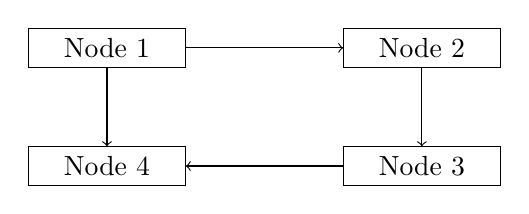
\begin{tikzpicture}
\draw (0,3) rectangle (2,3.5) node[pos=.5] {Node 1};
\draw (4,3) rectangle (6,3.5) node[pos=.5] {Node 2};

\draw (0,1.5) rectangle (2,2) node[pos=0.5] {Node 4};
\draw (4,1.5) rectangle (6,2) node[pos=0.5] {Node 3};

\draw[->] (2,3.25) -- (4,3.25);
\draw[<-] (2,1.75) -- (4,1.75);

\draw[->] (5,3) -- (5,2);
\draw[<-] (1,2) -- (1,3);

\end{tikzpicture}
\caption{Example for some circular dependency which might result in some deadlock depending on how the messages are send and received.}
\label{fig:mpi:circular}
\end{minipage}
\hfill
\begin{minipage}{0.45\linewidth}
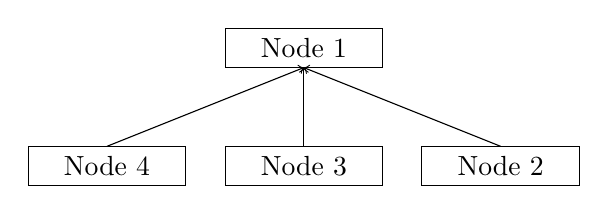
\begin{tikzpicture}
\draw (2.5,3) rectangle (4.5,3.5) node[pos=.5] {Node 1};

\draw (0,1.5) rectangle (2,2) node[pos=0.5] {Node 4};
\draw (2.5,1.5) rectangle (4.5,2) node[pos=0.5] {Node 3};
\draw (5,1.5) rectangle (7,2) node[pos=0.5] {Node 2};

\draw[->] (1,2) -- (3.5,3);
\draw[->] (3.5,2) -- (3.5,3);
\draw[->] (6,2) -- (3.5,3);

\end{tikzpicture}
\caption{A common principle is to use supervisor node the node with rank zero and this node is used to control messages with all nodes. }
\label{fig:mpi:rank}
\end{minipage}

\end{figure}


\newpage
\printendnotes